\documentclass[11pt, a4paper, jou]{apa7}
\setlength{\headheight}{14pt}
\usepackage[style=numeric, sorting=none]{biblatex}

\usepackage{hyperref}
\usepackage{url}
\usepackage{graphicx}
\usepackage{epstopdf}
\usepackage{amsmath}
\usepackage{float}

\addbibresource{Ref.bib}

\leftheader{ZEHAO WANG}

\linespread{1.5}
\title{Will it rain tomorrow? --- Course Report on Weather Prediction}
\shorttitle{BIOS-7650 COURSE PROJECT}
\author{Zehao Wang}
\authorsaffiliations{Master student in Statistics, Department of Mathematics}
\course{BIOS-7650 Statistical Learning in Data Science}
\professor{Dr.\ Li. }
\duedate{\today}
\abstract{In this report, we use the weather dataset from \href{https://www.kaggle.com/datasets/jsphyg/weather-dataset-rattle-package}{Kaggle} to predict the weather. We first modeled the data with logistic regression, achieving an accuracy of about $85.365\%$ on the test set. Then the SVM with kernel trick was used, achieving $85.272\%$ accuracy on the same test set. Finally, we used the current mainstream method of machine learning, neural networks, to achieve an accuracy of $85.9995\%$. And the code can be found in \href{https://github.com/Addasecond86/MS-Stat-Tulane/tree/main/Stat_Learning_in_Data_Analysis/Project/Code}{Github}. 
}
\begin{document}
\maketitle
\section{Methods}
Before we start fitting the data, we first need to clean it. For missing value, I dropped the subjects that had missing values in the variables \emph{RainToday} and \emph{RainTomorrow}. Because I have no good idea to fill in the missing values in these two variables. And I also dropped the subjects that contains missing value in categorical variables. For other continuous variables, it is not appropriate to fill the missing values with $0$, because variables such as temperature and barometric pressure cannot be $0$ even if they are missing. So I use the median of the current month to substitute the missing values of these continuous variables. 
\subsection{Logistic Regression}
    Logistic regression\cite{Berkson1944} is widely used in binary classification problems. Assume $p$ is the probability of rain tomorrow, then, for logistic regression, we have
    \begin{equation}
        \frac{p}{1-p}=\exp\left(\beta_0+\sum_{i=1}^{n}\beta_i x_i\right). 
    \end{equation}
    And we can estimate the coefficients $\beta_i$ by maximum likelihood estimation. 

    We first use all the variables except the date as predictor variables to predict whether it will rain tomorrow. Further, we use stepwise to explore whether the model can be further optimized. Akaike information criterion (AIC)\cite{Akaike1974} was used to see if any of the variables can be eliminated. AIC is a measure of the relative quality of statistical models for a given set of data. It is defined as following: 
    \begin{equation}
        \label{eq:AIC}
        {AIC} \,=\,2k-2\ln({\hat {L}}). 
    \end{equation}
    And $k$ is the number of estimated parameters in the model, $\hat{L}$ is the maximized value of the likelihood function for the model. So, the preferred model is the one with the minimum AIC value. 

    We also used Principal Component Analysis (PCA)\cite{Pearson1901} to extract features from the data. PCA is a method of reducing the dimensionality of data by transformation, which assumes that variables with higher variance carry more information. By reducing the dimensionality, we expect a significant increase in the classification accuracy. And because the absolute values of the variables are too different from each other, such as temperature and pressures. One is $20$, the other is more than $1000$. So, we should first transform the variables by \ref{eq:trans} and map them all to [0,1]. 
    \begin{equation}
        \label{eq:trans}
        X_{new} = \frac{X - X_{\min}}{X_{\max}- X_{\min}}
    \end{equation}
\subsection{SVM}
    Support Vector Machine (SVM) is a better method than logistic regression, it tries to maximize the margin between two different classes of data points. So it will have much lower risk on the test set. The optimization objectives of SVM are as follows: 
    \begin{equation}
        \min_{|w|}\ y_{i}(\mathbf {w} ^{\mathsf {T}}\mathbf {x} _{i}-b)\geq 1,\ i=1, \cdots, n
    \end{equation}
    When the data is not linearly separable, we can add soft margins to it. The optimization goal then becomes the following: 
    \begin{equation}
        \min_{|w|}\ \lambda |\mathbf {w}| ^{2}+{\frac {1}{n}}\sum _{i=1}^{n}\max \left(0,1-y_{i}(\mathbf {w} ^{\mathsf {T}}\mathbf {x} _{i}-b)\right). 
    \end{equation}
    After that, we can transform it into a dual problem and then estimate the parameters by gradient descent. 

    For nonlinear data sets, we can use the kernel trick to map the original data to the projection space. After that, we can separate them in the higher dimensional projection space using a linear hyperplane. By introducing different kernel functions, we can project them into different spaces. The common kernel functions are polynomial kernel functions and Gaussian kernel functions. 

\subsection{Neural Network}
    In the 21st century, network-based approaches are undoubtedly the mainstream of machine learning. Considering the complexity of the data, we only use a simple fully connected network with two hidden layers. Its structure is shown in figure \ref{fig:NN}. In this network, the activation functions of both fully connected hidden layers are ReLU\cite{Lu2020}, and it is shown as \ref{eq:ReLU}. It can solve the gradient disappearance or explosion problem in some extent. 
    \begin{equation}
        \label{eq:ReLU}
        ReLU(x) = \max(0,x)
    \end{equation}
    Also, Sigmoid is used as the activation function (\ref{eq:sigmoid}) in the output layer. Therefore, the final output we get is an output in $(0,1)$, and we consider values greater than $0.5$ as $1$, otherwise as $0$. 
    \begin{equation}
        \label{eq:sigmoid}
        Sigmoid(x) = \frac{1}{1+e^{-x}}
    \end{equation}
    The optimization algorithm for neural network parameters is Backpropagation\cite{goodfellow20166}. It uses the chain derivative rule to complete the update of the parameters. Since we are dealing with a binary classification problem, we use binary cross-entropy as the loss function. 
    \begin{equation}
        \label{eq:binary cross_entropy}
        L = -\frac{1}{n}\sum_{i=1}^{n}(y_i\ln(p_i)+(1-y_i)\ln(1-p_i))
    \end{equation}
    It can be seen that the more $p(y)$ matches with $y$, the closer the loss function is to $0$. On the contrary, it is infinite. 

\section{Results}

\subsection{Logistic Regression}
    Using $60\%$ as training set and $40\%$ as test set, logistic regression model with all the variables except the date has an accuracy of $85.365\%$ on the test set. And the accuracy on train set is $85.325\%$. The Confusion matrix is shown in figure~\ref{fig:logistic_confusion}. The accuracy and recall of this model are shown in table~\ref{tab:logistic_summary}. It can be seen that the accuracy ($0.88$) and recall ($0.95$) of the model are quite high with \emph{RainTomorrow} as \emph{No}. But it doesn't do well on data with \emph{RainTomorrow} as \emph{Yes}. 

    Next, we start from the full model and use AIC as a criterion to see if any variables can be excluded. The full process of stepwise is shown in table~\ref{tab:model_selection_aic}. Unfortunately, the AIC value of the full model is the smallest, so we cannot exclude any variables. 

\subsection{SVM}
Similarly, the data is divided by $60\%$ training set and $40\%$ test set. Using the SVM without kernel trick, the accuracy obtained on the test set is $85.272\%$. And the training accuracy is $85.170\%$. This result is basically the same as the logistic regression. It also shows that some of the data in our dataset are linearly inseparable. Its confusion matrix is shown in figure~\ref{fig:SVM_confusion}, and the accuracy and recall are shown in table~\ref{tab:SVM_summary}; It can also be seen that SVM has no improvement over logistic regression. 

The reason for no improvement in classification accuracy may be that the data itself is linearly inseparable. So we try to introduce two kernel functions (polynomial and Gaussian). The results are shown in figure~\ref{fig:SVM_poly_confusion}, \ref{fig:SVM_gauss_confusion} and table~\ref{tab:SVM_poly_summary}, \ref{tab:SVM_gauss_summary}. However, based on the classification results, the accuracy of both methods on the test set is slightly lower. This is probably because the two kernel functions cannot separate these two classes of data. 

However, in general, SVM should perform better, so we tried to use PCA to extract features first, and then use the model to classify the data. Using PCA, we chose to retain $85\%$ of the information, and we reduced the original 114-dimensional data to 64 dimensions. The classification results on this data are shown in table \ref{tab:Logit_PCA_summary}, \ref{tab:SVM_PCA_summary}, \ref{tab:SVM_poly_PCA_summary}, \ref{tab:SVM_gauss_PCA_summary}. 
Unfortunately, however, these results indicate that there is no significant increase in accuracy on the test set. Unfortunately, however, these results indicate that the accuracy on the test set does not increase, but decreases slightly. At the same time, several SVM-based models show a further increase in training accuracy (SVM polynomial, train accuracy: $87.048\%$, test accuracy: $84.377\%$; SVM gaussian: train accuracy: $86.711\%$, test accuracy: $84.789\%$), but a decrease in test accuracy, indicating that overfitting has occurred. This indicates that PCA cannot lead to further improvement of accuracy. 



\subsection{Neural Network}
We mapped the data to $(0,1)$ and started training. First, the network was trained with ¥ Epochs. The loss of the model on the test set and the loss on the validation set during the training process are shown in figure \ref{fig:NN_process_50}. It can be seen that, although the training loss keeps decreasing, the loss on the validation set stops decreasing after $20$ Epochs. It even starts to increase after $30$ Epochs. This indicates that the overfitting starts after $20$ Epochs. Therefore, we retrain a network with only $20$ Epochs. And the training process is shown as figure \ref{fig:NN_process_20}. It can be seen from the figure that no overfitting has occurred. The performance of this network on the test set is shown in figure \ref{fig:FC_confusion_matrix} and table \ref{tab:FC_summary}. In the end, we obtained an accuracy of $85.9995\%$ on the test set. This accuracy is a little higher than either logistic regression or SVM. 

\section{Discussion}

As you can see, we use three different approaches. But the results are basically the same, that is, we can only achieve an accuracy of less than $86\%$ at most. This seems very frustrating, because it means that the error rate has about $15\%$. This means that on average we will be wrong one day out of a week. 

However, this is about the level of accuracy of current weather predictions. You can see the accuracy of the weather predictions for New Orleans last year on this \href{https://www.forecastadvisor.com/Louisiana/NewOrleans/70112/}{website}. As shown in figure \ref{fig:weather_prediction_nola}, this website shows that the highest channel for 2021 weather prediction accuracy in the New Orleans area is just $85\%$. 

In addition, we can see that the accuracy and recall of the three models are relatively high for the forecast of not raining. For the forecast of raining, the accuracy and recall are lower. This means that when the weather prediction says it will not rain, then it is very likely that it will not rain. But when the prediction says it will rain, then there is also a chance that it will not rain. Therefore, we can see that weather prediction nowadays does not predict whether raining or not directly, but uses a rainfall probability instead. 

\printbibliography 
\clearpage
\appendix
\section{Figures and Tables}
\begin{figure}[h]
    \centering
    \caption{Confusion matrix of logistic regression model}\label{fig:logistic_confusion}
    \includegraphics[width=.45\textwidth]{figures/Logit_confusion_matrix.eps}
\end{figure}

\begin{figure}[h]
    \centering
    \caption{Confusion matrix of SVM}\label{fig:SVM_confusion}
    \includegraphics[width=.45\textwidth]{figures/SVM_confusion_matrix.eps}
\end{figure}

\begin{figure}[h]
    \centering
    \caption{Confusion matrix of SVM with polynomial kernel function}\label{fig:SVM_poly_confusion}
    \includegraphics[width=.45\textwidth]{figures/SVM_poly_confusion_matrix.eps}
\end{figure}

\begin{figure}[h]
    \centering
    \caption{Confusion matrix of SVM with gaussian kernel function}\label{fig:SVM_gauss_confusion}
    \includegraphics[width=.45\textwidth]{figures/SVM_gauss_confusion_matrix.eps}
\end{figure}

\begin{table}[h]
    \centering
    \caption{Logistic regression model summary}
    \label{tab:logistic_summary}
    \resizebox{\columnwidth}{!}{%
    \begin{tabular}{rrrrr}
    \hline
                 & precision & recall & f1-score & support \\ \hline
    Not Raining  & 0.87      & 0.95   & 0.91     & 38571   \\
    Raining      & 0.73      & 0.53   & 0.62     & 10913    \\
    accuracy     &           &        & 0.85     & 49484   \\
    macro avg    & 0.80      & 0.74   & 0.76     & 49484   \\
    weighted avg & 0.84      & 0.85   & 0.84     & 49484   \\ \hline
    \end{tabular}%
    }
\end{table}

\begin{table}[h]
    \centering
    \caption{SVM summary}
    \label{tab:SVM_summary}
    \resizebox{\columnwidth}{!}{%
    \begin{tabular}{rrrrr}
    \hline
                 & precision & recall & f1-score & support \\ \hline
    Not Raining  & 0.87      & 0.95   & 0.91     & 38571   \\
    Raining      & 0.74      & 0.51   & 0.61     & 10913    \\
    accuracy     &           &        & 0.85     & 49484   \\
    macro avg    & 0.81      & 0.73   & 0.76     & 49484   \\
    weighted avg & 0.84      & 0.85   & 0.84     & 49484   \\ \hline
    \end{tabular}%
    }
\end{table}

\begin{table}[h]
    \centering
    \caption{SVM with polynomial kernel function summary}
    \label{tab:SVM_poly_summary}
    \resizebox{\columnwidth}{!}{%
    \begin{tabular}{rrrrr}
    \hline
                 & precision & recall & f1-score & support \\ \hline
    Not Raining  & 0.85      & 0.96   & 0.91     & 38571   \\
    Raining      & 0.76      & 0.41   & 0.61     & 10913    \\
    accuracy     &           &        & 0.84     & 49484   \\
    macro avg    & 0.81      & 0.69   & 0.72     & 49484   \\
    weighted avg & 0.83      & 0.84   & 0.82     & 49484   \\ \hline
    \end{tabular}%
    }
\end{table}

\begin{table}[h]
    \centering
    \caption{SVM with gaussian kernel function summary}
    \label{tab:SVM_gauss_summary}
    \resizebox{\columnwidth}{!}{%
    \begin{tabular}{rrrrr}
    \hline
                 & precision & recall & f1-score & support \\ \hline
    Not Raining  & 0.85      & 0.97   & 0.90     & 38571   \\
    Raining      & 0.79      & 0.37   & 0.51     & 10913    \\
    accuracy     &           &        & 0.84     & 49484   \\
    macro avg    & 0.82      & 0.67   & 0.71     & 49484   \\
    weighted avg & 0.83      & 0.84   & 0.82     & 49484   \\ \hline
    \end{tabular}%
    }
\end{table}
    
\begin{table}[h]
    \centering
    \caption{Model selection for logistic regression with AIC as criterion}
    \label{tab:model_selection_aic}
    \begin{tabular}{lrrr}
    \hline
                   & Df & Deviance & AIC                          \\ \hline
    Full Model     &    & 84120    & {\color[HTML]{FE0000} 84338} \\
    -Temp3pm       & 1  & 84130    & 84346                        \\
    -Cloud9am      & 1  & 84131    & 84347                        \\
    -Evaporation   & 1  & 84131    & 84347                        \\
    -Humidity9am   & 1  & 84135    & 84351                        \\
    -WindGustDir   & 15 & 84168    & 84356                        \\
    -MinTemp       & 1  & 84148    & 84364                        \\
    -Temp9am       & 1  & 84152    & 84368                        \\
    -WindSpeed9am  & 1  & 84174    & 84390                        \\
    -Rainfall      & 1  & 84175    & 84391                        \\
    -MaxTemp       & 1  & 84219    & 84435                        \\
    -WindDir9am    & 15 & 84311    & 84499                        \\
    -WindDir3pm    & 15 & 84324    & 84512                        \\
    -WindSpeed3pm  & 1  & 84471    & 84687                        \\
    -RainToday     & 1  & 84491    & 84707                        \\
    -Sunshine      & 1  & 84538    & 84754                        \\
    -Cloud3pm      & 1  & 84799    & 85015                        \\
    -Pressure9am   & 1  & 84819    & 85035                        \\
    -Pressure3pm   & 1  & 85390    & 85606                        \\
    -Location      & 46 & 86542    & 86668                        \\
    -WindGustSpeed & 1  & 87585    & 87801                        \\
    -Humidity3pm   & 1  & 87949    & 88165                        \\ \hline
    \end{tabular}
\end{table}

\begin{table}[h]
    \centering
    \caption{Logistic regression model using PCA summary}
    \label{tab:Logit_PCA_summary}
    \resizebox{\columnwidth}{!}{%
    \begin{tabular}{rrrrr}
    \hline
                 & precision & recall & f1-score & support \\ \hline
    Not Raining  & 0.86      & 0.94   & 0.90     & 38571   \\
    Raining      & 0.69      & 0.45   & 0.54     & 10913    \\
    accuracy     &           &        & 0.83     & 49484   \\
    macro avg    & 0.77      & 0.70   & 0.72     & 49484   \\
    weighted avg & 0.82      & 0.83   & 0.82     & 49484   \\ \hline
    \end{tabular}%
    }
\end{table}

\begin{table}[h]
    \centering
    \caption{SVM using PCA summary}
    \label{tab:SVM_PCA_summary}
    \resizebox{\columnwidth}{!}{%
    \begin{tabular}{rrrrr}
    \hline
                 & precision & recall & f1-score & support \\ \hline
    Not Raining  & 0.85      & 0.95   & 0.90     & 38571   \\
    Raining      & 0.71      & 0.41   & 0.52     & 10913    \\
    accuracy     &           &        & 0.83     & 49484   \\
    macro avg    & 0.78      & 0.68   & 0.71     & 49484   \\
    weighted avg & 0.82      & 0.83   & 0.82     & 49484   \\ \hline
    \end{tabular}%
    }
\end{table}

\begin{table}[h]
    \centering
    \caption{SVM with polynomial kernel function and using PCA summary}
    \label{tab:SVM_poly_PCA_summary}
    \resizebox{\columnwidth}{!}{%
    \begin{tabular}{rrrrr}
    \hline
                 & precision & recall & f1-score & support \\ \hline
    Not Raining  & 0.86      & 0.96   & 0.91     & 38571   \\
    Raining      & 0.74      & 0.45   & 0.56     & 10913    \\
    accuracy     &           &        & 0.84     & 49484   \\
    macro avg    & 0.80      & 0.70   & 0.73     & 49484   \\
    weighted avg & 0.83      & 0.84   & 0.83     & 49484   \\ \hline
    \end{tabular}%
    }
\end{table}

\begin{table}[h]
    \centering
    \caption{SVM with gaussian kernel function and using PCA summary}
    \label{tab:SVM_gauss_PCA_summary}
    \resizebox{\columnwidth}{!}{%
    \begin{tabular}{rrrrr}
    \hline
                 & precision & recall & f1-score & support \\ \hline
    Not Raining  & 0.86      & 0.96   & 0.91     & 38571   \\
    Raining      & 0.75      & 0.47   & 0.57     & 10913    \\
    accuracy     &           &        & 0.83     & 49484   \\
    macro avg    & 0.81      & 0.71   & 0.74     & 49484   \\
    weighted avg & 0.84      & 0.85   & 0.83     & 49484   \\ \hline
    \end{tabular}%
    }
\end{table}

\begin{figure}[h]
    \centering
    \caption{Neural network structure}\label{fig:NN}
    \includegraphics[width=.3\textwidth]{figures/Network_structure.png}
\end{figure}

\begin{figure}[h]
    \centering
    \caption{Training process with epoch $=$ 50. }\label{fig:NN_process_50}
    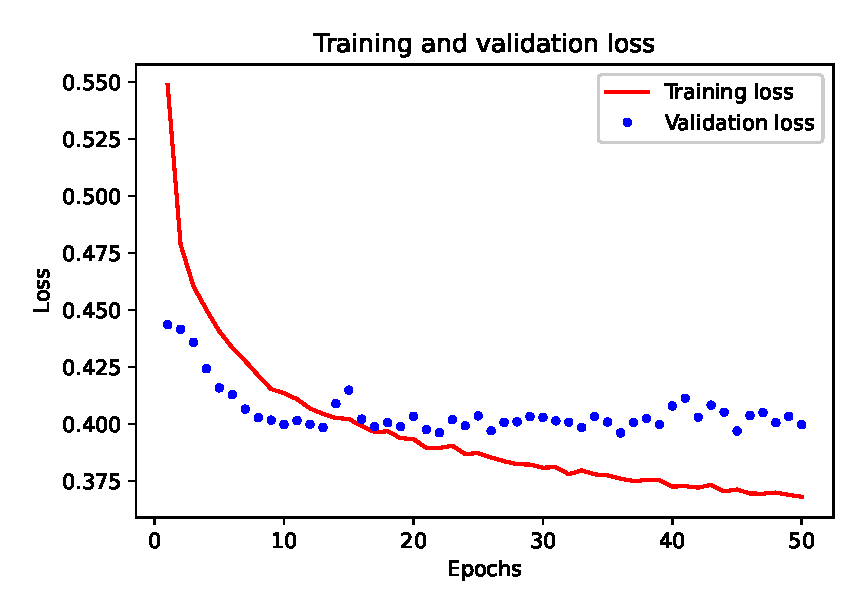
\includegraphics[width=.45\textwidth]{figures/error_50.eps}
\end{figure}

\begin{figure}[h]
    \centering
    \caption{Training process with epoch $=$ 20. }\label{fig:NN_process_20}
    \includegraphics[width=.45\textwidth]{figures/error_20.eps}
\end{figure}

\begin{figure}[h]
    \centering
    \caption{Confusion matrix of Neural Network}\label{fig:FC_confusion_matrix}
    \includegraphics[width=.45\textwidth]{figures/FC_confusion_matrix.eps}
\end{figure}

\begin{table}[h]
    \centering
    \caption{Neural Network summary}
    \label{tab:FC_summary}
    \resizebox{\columnwidth}{!}{%
    \begin{tabular}{rrrrr}
    \hline
                 & precision & recall & f1-score & support \\ \hline
    Not Raining  & 0.89      & 0.93   & 0.91     & 38571   \\
    Raining      & 0.71      & 0.61   & 0.66     & 10913    \\
    accuracy     &           &        & 0.86     & 49484   \\
    macro avg    & 0.80      & 0.77   & 0.78     & 49484   \\
    weighted avg & 0.85      & 0.86   & 0.86     & 49484   \\ \hline
    \end{tabular}%
    }
\end{table}

\begin{figure}[h]
    \centering
    \caption{Weather prediction accuracy for New Orleans in 2021}\label{fig:weather_prediction_nola}
    \includegraphics[width=.45\textwidth]{figures/Weather2021.png}
\end{figure}

\end{document}